\begin{pastexam}[label={px:ncku-107-ee-ds-09}]{成大電機所 107 學年度 問答題第 5 題}
（問答）

\textbf{5. (14 pts) Spanning Tree:}

Find the minimal cost spanning tree according to (a) Kruskal's algorithm and (b) the Sollin's
Algorithm, respectively. Please show the result in each iteration of the algorithm.

\begin{center}
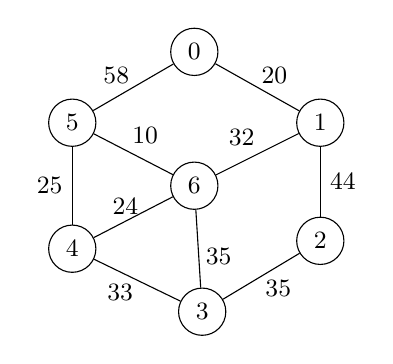
\begin{tikzpicture}[v/.style={draw,circle,minimum size=6mm,inner sep=0pt},font=\small]
  \node[v] (0) at (0,0) {0};
  \node[v] (5) at (-1.55,-0.9) {5};
  \node[v] (1) at (1.6,-0.9) {1};
  \node[v] (6) at (0,-1.7) {6};
  \node[v] (4) at (-1.55,-2.5) {4};
  \node[v] (2) at (1.6,-2.4) {2};
  \node[v] (3) at (0.1,-3.3) {3};
  \draw (0) -- node[above left=-2pt] {58} (5);
  \draw (0) -- node[above right=-2pt] {20} (1);
  \draw (5) -- node[above right=-1pt,pos=0.4] {10} (6);
  \draw (6) -- node[above left=-1pt,pos=0.55] {32} (1);
  \draw (5) -- node[left] {25} (4);
  \draw (4) -- node[above=-1pt,pos=0.4] {24} (6);
  \draw (1) -- node[right] {44} (2);
  \draw (6) -- node[right=-1pt,pos=0.6] {35} (3);
  \draw (4) -- node[below left=-2pt] {33} (3);
  \draw (3) -- node[below right=-2pt] {35} (2);
\end{tikzpicture}
\end{center}
\end{pastexam}

\begin{pastsoln}
兩種方法得到同一棵最小生成樹，邊是 $(5,6)$、$(0,1)$、$(4,6)$、$(1,6)$、$(3,4)$、$(2,3)$，總成本
$10 + 20 + 24 + 32 + 33 + 35 = 154$。 圖有 $7$ 個頂點、$10$ 條邊，要選 $6$ 條。 有兩條權重 $35$ 的邊，照資結書
第~24.1.7~節的約定，同權重時比較端點：$(2,3) \prec (3,6)$。

\textbf{(a) Kruskal}（資結書虛擬碼~24.2）：邊由小到大排好，依序看，兩端不在同一棵樹就選，否則略過。
\begin{center}
\small
\begin{tabular}{rcrll}
\toprule
步 & 邊 & 成本 & 結果 & 選邊後的樹（只列兩個以上頂點的） \\
\midrule
1 & $(5,6)$ & 10 & 選 & $\{5,6\}$ \\
2 & $(0,1)$ & 20 & 選 & $\{5,6\}$、$\{0,1\}$ \\
3 & $(4,6)$ & 24 & 選 & $\{4,5,6\}$、$\{0,1\}$ \\
4 & $(4,5)$ & 25 & 略過：4、5 已連通（4--6--5），會成環 & 同上 \\
5 & $(1,6)$ & 32 & 選 & $\{0,1,4,5,6\}$ \\
6 & $(3,4)$ & 33 & 選 & $\{0,1,3,4,5,6\}$ \\
7 & $(2,3)$ & 35 & 選，已滿 $6$ 條，停止 & $\{0,1,2,3,4,5,6\}$ \\
\bottomrule
\end{tabular}
\end{center}
沒看到的邊是 $(3,6)$ 35、$(1,2)$ 44、$(0,5)$ 58。 就算先看 $(3,6)$，那時 $3$ 已經經由 $(3,4)$ 接上 $6$ 那棵樹，
會被略過，結果不變。

\textbf{(b) Sollin}（資結書虛擬碼~24.6）：每一回合，每一棵樹各自挑一條連到別棵樹的最輕邊，全部加入後合併。
\begin{itemize}
\item \textbf{第 1 回合}：一開始每個頂點自己一棵樹。
\begin{center}
\small
\begin{tabular}{cll}
\toprule
樹 & 連出去的邊 & 挑的最輕邊 \\
\midrule
$\{0\}$ & $(0,1)$ 20、$(0,5)$ 58 & $(0,1)$ 20 \\
$\{1\}$ & $(0,1)$ 20、$(1,6)$ 32、$(1,2)$ 44 & $(0,1)$ 20 \\
$\{2\}$ & $(2,3)$ 35、$(1,2)$ 44 & $(2,3)$ 35 \\
$\{3\}$ & $(3,4)$ 33、$(2,3)$ 35、$(3,6)$ 35 & $(3,4)$ 33 \\
$\{4\}$ & $(4,6)$ 24、$(4,5)$ 25、$(3,4)$ 33 & $(4,6)$ 24 \\
$\{5\}$ & $(5,6)$ 10、$(4,5)$ 25、$(0,5)$ 58 & $(5,6)$ 10 \\
$\{6\}$ & $(5,6)$ 10、$(4,6)$ 24、$(1,6)$ 32、$(3,6)$ 35 & $(5,6)$ 10 \\
\bottomrule
\end{tabular}
\end{center}
挑到的邊去掉重複是 $(0,1)$、$(2,3)$、$(3,4)$、$(4,6)$、$(5,6)$，加入後剩兩棵樹：$\{0, 1\}$ 和 $\{2, 3, 4, 5, 6\}$。
\item \textbf{第 2 回合}：兩棵樹之間的邊有 $(1,6)$ 32、$(1,2)$ 44、$(0,5)$ 58，兩棵樹都挑 $(1,6)$ 32。 加入後只剩一棵
樹，結束。
\end{itemize}
Sollin 兩個回合就完成（每回合樹的個數至少減半，資結書定理~24.8），選到的六條邊和 Kruskal 相同。 這張圖的
最小生成樹是唯一的：唯一的同權重邊對 $(2,3)$、$(3,6)$ 裡，$(3,6)$ 在 $3$ 和 $6$ 之間的環
$3\!-\!4\!-\!6\!-\!3$ 上是最重的邊（$35 > 33, 24$），不可能在任何最小生成樹裡。

最後的樹（粗線）：
\begin{center}
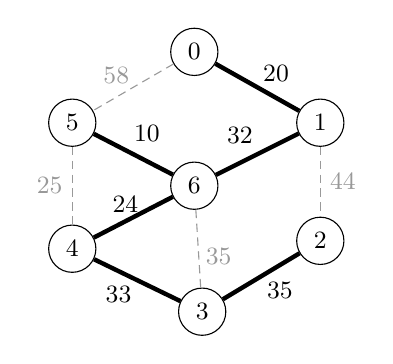
\begin{tikzpicture}[v/.style={draw,circle,minimum size=6mm,inner sep=0pt},font=\small,
  t/.style={line width=1.6pt}, n/.style={densely dashed,black!40}]
  \node[v] (0) at (0,0) {0};
  \node[v] (5) at (-1.55,-0.9) {5};
  \node[v] (1) at (1.6,-0.9) {1};
  \node[v] (6) at (0,-1.7) {6};
  \node[v] (4) at (-1.55,-2.5) {4};
  \node[v] (2) at (1.6,-2.4) {2};
  \node[v] (3) at (0.1,-3.3) {3};
  \draw[n] (0) -- node[above left=-2pt] {58} (5);
  \draw[t] (0) -- node[above right=-2pt] {20} (1);
  \draw[t] (5) -- node[above right=-1pt,pos=0.4] {10} (6);
  \draw[t] (6) -- node[above left=-1pt,pos=0.55] {32} (1);
  \draw[n] (5) -- node[left] {25} (4);
  \draw[t] (4) -- node[above=-1pt,pos=0.4] {24} (6);
  \draw[n] (1) -- node[right] {44} (2);
  \draw[n] (6) -- node[right=-1pt,pos=0.6] {35} (3);
  \draw[t] (4) -- node[below left=-2pt] {33} (3);
  \draw[t] (3) -- node[below right=-2pt] {35} (2);
\end{tikzpicture}
\end{center}
\end{pastsoln}
